% --- Template for thesis / report with tktltiki2 class ---
%
% last updated 2013/02/15 for tkltiki2 v1.02

\documentclass[finnish]{tktltiki2}

% tktltiki2 automatically loads babel, so you can simply
% give the language parameter (e.g. finnish, swedish, english, british) as
% a parameter for the class: \documentclass[finnish]{tktltiki2}.
% The information on title and abstract is generated automatically depending on
% the language, see below if you need to change any of these manually.
%
% Class options:
% - grading                 -- Print labels for grading information on the front page.
% - disablelastpagecounter  -- Disables the automatic generation of page number information
%                              in the abstract. See also \numberofpagesinformation{} command below.
%
% The class also respects the following options of article class:
%   10pt, 11pt, 12pt, final, draft, oneside, twoside,
%   openright, openany, onecolumn, twocolumn, leqno, fleqn
%
% The default font size is 11pt. The paper size used is A4, other sizes are not supported.
%
% rubber: module pdftex

% --- General packages ---

\usepackage[utf8]{inputenc}
\usepackage[T1]{fontenc}
\usepackage{lmodern}
\usepackage{microtype}
\usepackage{amsfonts,amsmath,amssymb,amsthm,booktabs,color,enumitem,graphicx}
\usepackage[pdftex,hidelinks]{hyperref}

% Automatically set the PDF metadata fields
\makeatletter
\AtBeginDocument{\hypersetup{pdftitle = {\@title}, pdfauthor = {\@author}}}
\makeatother

% --- Language-related settings ---
%
% these should be modified according to your language

% babelbib for non-english bibliography using bibtex
\usepackage[fixlanguage]{babelbib}
\selectbiblanguage{finnish}

% add bibliography to the table of contents
\usepackage[nottoc]{tocbibind}
% tocbibind renames the bibliography, use the following to change it back
\settocbibname{Lähteet}

% --- Theorem environment definitions ---

\newtheorem{lau}{Lause}
\newtheorem{lem}[lau]{Lemma}
\newtheorem{kor}[lau]{Korollaari}

\theoremstyle{definition}
\newtheorem{maar}[lau]{Määritelmä}
\newtheorem{ong}{Ongelma}
\newtheorem{alg}[lau]{Algoritmi}
\newtheorem{esim}[lau]{Esimerkki}

\theoremstyle{remark}
\newtheorem*{huom}{Huomautus}


% --- tktltiki2 options ---
%
% The following commands define the information used to generate title and
% abstract pages. The following entries should be always specified:

\title{Ohjelmiston kompleksisuuden mittaaminen}
\author{Janne Haapsaari}
\date{\today}
\level{Referaatti}

% The following can be used to specify keywords and classification of the paper:

\keywords{syklomaattinen kompleksisuus, ohjelmiston ohjausvuo}

% classification according to ACM Computing Classification System (http://www.acm.org/about/class/)
% This is probably mostly relevant for computer scientists
% uncomment the following; contents of \classification will be printed under the abstract with a title
% "ACM Computing Classification System (CCS):"
% \classification{}

% If the automatic page number counting is not working as desired in your case,
% uncomment the following to manually set the number of pages displayed in the abstract page:
%
% \numberofpagesinformation{16 sivua + 10 sivua liitteissä}
%
% If you are not a computer scientist, you will want to uncomment the following by hand and specify
% your department, faculty and subject by hand:
%
% \faculty{Matemaattis-luonnontieteellinen}
% \department{Tietojenkäsittelytieteen laitos}
% \subject{Tietojenkäsittelytiede}
%
% If you are not from the University of Helsinki, then you will most likely want to set these also:
%
% \university{Helsingin Yliopisto}
% \universitylong{HELSINGIN YLIOPISTO --- HELSINGFORS UNIVERSITET --- UNIVERSITY OF HELSINKI} % displayed on the top of the abstract page
% \city{Helsinki}
%


\begin{document}

% --- Front matter ---

\frontmatter      % roman page numbering for front matter

\maketitle        % title page

\tableofcontents  % table of contents

% --- Main matter ---

\mainmatter       % clear page, start arabic page numbering

\section{Johdanto}

% Write some science here.
Eräs ohjelmistoteollisuuden kriittisistä tutkimuskysymyksistä on selvittää kuinka ohjelmistot voidaan jakaa helpommin testattaviin ja ylläpidettäviin komponentteihin. Ohjelmiston testattavuus ja ylläpidettävyys ovat keskeisiä asioita ohjelmistoteollisuudessa. Usein jopa puolet ohjelmistokehityksestä on testausta ja suurin osan projektin budjetista kuluu ylläpitoon. Perinteiset menetelmät ohjelmiston modularisaation varmistamiseen pohjautuvat lähdekoodin fyysisen koon, kuten koodirivien määrän, rajoittamiseen. Menetelmä ei sellaisenaan ole riittävä, sillä koodiriveiltään vähäinen moduuli voi sisältää valtavan määrän kontrollipolkuja (control path). Kontrollipolkujen määrän on havaittu korreloivan ohjelmiston monimutkaisuuden kanssa. Suuri kontrollipolkujen määrä vaikeuttaa ohjelmiston ylläpidettävyyttä ja testattavuutta.

McCabe esittelee artikkelissa ''A Complexity Measure''~\cite{McGabe} matemaattisen menetelmän ohjelmiston kompleksisuuden mittaamiseen. Menetelmä tarjoaa laskennallisen pohjan ohjelmiston monimutkaisuuden arvioimiseksi ja auttaa ohjelmistokehittäjiä tunnistamaan vaikeasti ylläpidettävät ja testattavat osat. Menetelmässä ohjelmiston ohjausvuon (program control flow) esitetään suunnattuna verkkona (directed graph).

\section{Kompleksisuuden mittaaminen}

McCaben menetelmä pyrkii mittaamaan ohjelmiston kompleksisuutta ja rajoittamaan kontrollipolkujen määrää ohjelmistossa. Kontrollipolkujen määrän laskeminen ei kuitenkaan ole yksiselitteistä, sillä palautuva kontrollipolku saattaa kasvattaa kontrollipolkujen määrän äärettömän suureksi. Tämä ei kuitenkaan muodostu ongelmaksi, sillä arvioitaessa kompleksisuutta ohjelmiston kantapolkujen (basic path) määrä on kokonaismäärää käytännöllisempi suure. Kantapolut ovat joukko kontrollipolkuja ohjelmistossa, joiden yhdistelmillä voidaan muodostaa kaikki kontrollipolut. McCabe kutsuu menetelmää syklomaattiseksi kompleksisuudeksi (cyclomatic complexity).

%\section{Syklomaattinen kompleksisuus}

McCabe esittää määritelmän ja lemman, joiden soveltamista hän havainnolistaa esimerkkien avulla.

\begin{maar}\label{maar1}
  Yleisesti verkon G syklomaattinen kompleksisuus v(G) voidaan laskea kaavalla
  \begin{equation}\label{eq}
    v(G) = e - n + 2p.
  \end{equation}

  Kaavassa \eqref{eq} $n$ on verkon solmujen määrä, $e$ verkon särmien määrä sekä $p$ verkon yhdistettyjen komponenttien määrä.
\end{maar}

\newpage

\begin{lem}\label{lem}
  Vahvasti yhtenäisessä verkossa (strongly connected graph) G syklomaattinen kompleksisuus on sama kuin lineaarisesti riippumattomien polkujen (linearly independent circuit) maksimimäärä. Tällöin syklomaattisen kompleksisuuden laskeva kaava muuttuu muotoon
  \begin{equation}\label{eq2}
    v(G) = e - n + p.
  \end{equation}
  Kaavassa \eqref{eq2} $n$ on verkon solmujen määrä, $e$ verkon särmien (edge) määrä ja $p$ verkon yhdistettyjen komponenttien määrä.
\end{lem}

Syklomaattinen kompleksisuus esitetään muodostamalla ohjelmistosta suunnattu verkko. Verkon jokainen solmu (node) kuvaa ohjelmakoodin osaa, jossa ohjausvuo etenee lineaarisesti. Verkon kaaret kuvaavat ohjausvuon haarautumista eri kontrollipoluille. Verkon lähtösolmu (entry node) ja maalisolmu (exit node) ovat yksilöityjä. Oletus on että jokaiseen solmuun voidaan päästä lähtösolmusta sekä jokaisesta solmusta voidaan päästä maalisolmuun. Tällaisen verkon klassinen nimitys on ohjelmiston vuokaavio (program control graph).

Seuraavassa esimerkissä satunnaisen ohjelmiston vuokaavion on esitetty verkkona $G$, jonka lähtösolmu on solmu $a$ ja maalisolmu on solmu $f$.

\centerline{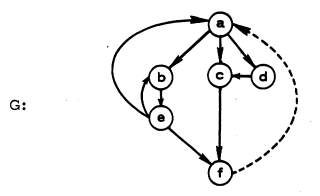
\includegraphics[scale=0.7]{verkko.png}}

Jos kuvittelemme kaaren verkon maalisolmusta lähtösolmuun, saamme muodostettua esimerkin verkosta vahvasti yhtenäisen verkon. Vahvasti yhtenäisessä verkossa jokaisesta solmusta on polku jokaiseen toiseen solmuun. Lemma \eqref{lem} siis pätee esimerkin verkkoon $G$. Siten lineaarisesti riippumattomien polkujen (linearly independent path) suurin mahdollinen määrä verkossa $G$ on 9 - 6 + 2 = 5.

Voimme siis valita esimerkiksi seuraavat viisi lineaarisesti riippumatonta polkua verkosta $G$.

\centerline{B1: \{(abefa), (beb), (abea), (acfa), (adcfa)\}.}

Lineaarisesti riippumattomien polkujen joukko B1 on kantajoukko (basis of set), jonka alkioiden yhdistelminä voidaan esittää kaikki polut verkon G sisällä. Esimerkiksi polku (abeabebebef) voidaan esittää muodossa (abea) + 2(beb) + (abefa).
\newpage
Syklomaattisen kompleksisuuden arvolla on lisäksi seuraavat ominaisuudet
\begin{enumerate}
  \item $ v(G) \geq 1. $
  \item v(G) on yhtä suuri kuin lineaaristen riippumattomien polkujen maksimimäärä.
  \item Toiminnallisten lausekkeiden lisääminen tai poistaminen ei vaikuta v(G):n arvoon.
  \item Verkossa G on vain yksi polku, jos $v(G) = 1$.
  \item Kaaren lisääminen verkkoon G kasvattaa v(G) arvoa yhdellä.
  \item v(G):n arvo riippuu ainoastaan verkon G kontrollirakenteista.
\end{enumerate}

Mitä suurempi syklomaattisen kompleksisuuden arvo on, sitä monimutkaisempi ohjelmisto on kyseessä. Kontrollipolkujen kokonaismäärän sijaan ohjelmiston kompleksisuutta arvioitaessa voidaan keskittyä itsenäisesti riippumattomien polkujen määrään (v(G)), rajoittaa sen kokoa ja käyttää syklomaattista kompleksisuutta pohjana testauksessa.

\section{Kokemukset kompleksisuuden mittaamisesta}

Tutkimusta helpottaakseen McCabe on kehittänyt FLOW ohjelman FORTRAN ohjelmakoodin analysointia varten. FLOW automatisoi ohjelmiston vuokaavion luomisen, laskee syklomaattisen kompleksisuuden ja tulostaa vuokaavion yhteysmatriisin (reachability matrix). Automatisoinnin seurauksena McCabe kykenee aikaisempaa huomattavasti nopeammin arvioimaan ohjelmistojen monimutkaisuutta.

Artikkelissa McCabe esittää lukuisia käytössä olevien ohjelmistojen vuokaaviota. Tutkimustulosten perusteella on havaittu läheinen korrelaatio korkean syklomaattisen kompleksisuusarvon ja ohjelmiston luotettavuuden välillä. Tulosten perusteella syklomaattisen kompleksisuuden arvon ylärajaksi hän suosittelee arvoa kymmenen. Arvon noustessa yli kymmenen ohjelmiston osa tulisi jakaa osiin tai suunnitella uudelleen. Tarkoituksena on pitää ohjelmiston komponentit koko pienenä, jotta kaikki itsenäiset kontrollipolut voitaisiin testata. Tilanteissa, joissa ohjelmistossa jakaudutaan suureen määrään itsenäisiä kontrollirakenteita, suositeltu arvo vaikuttaa kohtuuttoman pieneltä. Esimerkiksi strukturoidussa ohjelmoinnissa (structured programming) tyypillisen suuren case-lausekkeen tapauksessa McCabe sallii arvon ylittämisen.

\section{Johtopäätökset}

Syklomaattisen kompleksisuuden arvon on havaittu korreloivan ohjelmiston monimutkaisuuden kanssa. Kokemuksen mukaan arvosta on eniten apua tilanteissa, joissa ohjelmoijaa vaaditaan dokumentoimaan ohjelman vuokaavio.

Jos testattavan ohjelmiston syklomaattinen kompleksisuus $v$ on suurempi kuin testattujen polkujen määrä $tp$, on jokin seuraavista totta
\begin{itemize}
  \item Ohjelmassa on lisää testausta vaativia kontrollipolkuja.
  \item Ohjelmavuo on yksinkertaistettavissa, eli kontrollipolkujen määrä on vähennettävissä $v-tp$ verran.
  \item Ohjelmiston osia on pelkistettävissä käyttäen inline-ohjelmakoodia (in line code). Tällöin ohjelmiston kompleksisuus on lisääntynyt ohjelmakoodin fyysisten rajoitteiden takia.
\end{itemize}

Testattujen polkujen määrää verrattaessa syklomaattiseen kompleksisuuteen löydetään usein uusia testaamattomia kontrollipolkuja. On huomautettava, että syklomaattinen kompleksisuus v on vain vähimmäismäärä itsenäisiä polkuja jotka on testattava. On yleistä, että testattavia polkuja on enemmän. Syklomaattinen kompleksisuus, kuten mikään muukaan testausmenetelmä, ei takaa virheetöntä ohjelmistoa, vain ainoastaan saattaa auttaa virheiden löytymisessä ja siten parantaa ohjelmiston laatua.


% --- References ---
%
% bibtex is used to generate the bibliography. The babplain style
% will generate numeric references (e.g. [1]) appropriate for theoretical
% computer science. If you need alphanumeric references (e.g [Tur90]), use
%
% \bibliographystyle{babalpha-lf}
%
% instead.
\bibliographystyle{babplain-lf}
\bibliography{references-fi}


% --- Appendices ---

% uncomment the following

% \newpage
% \appendix
%
% \section{Esimerkkiliite}

\end{document}
